% Provenance (never printed): see sources/outline_sources.md (Year 3:
% energy-balance models, the one-layer model recalled; ice-albedo feedback
% and multiple equilibria; how general circulation models are built and
% evaluated).
% Brief: sources/book5/BRIEFS.md, ch. 22. Curves from
% figdata/bachelor-3/budyko_sellers.py (the zero-dimensional model and
% Budyko's latitudinal model; the brief's ebm_0d is folded into it) and
% two_layer.py. Exercise and problem values in the Book 5 scratch calculator
% calc/ch22.py. The model planet, model X and the ensemble of exercise 12 are
% invented.
\chapter{Klimaatmodellen}\label{ch:b3:climate-models}

Neem het zonlicht dat de Aarde bereikt, \qty{340}{W/m^2} gemiddeld over de
bol, en een wet voor de infrarode straling die de Aarde naar de ruimte terugstuurt, afgestemd op
dertig jaar reanalyse van de waarnemingen. Laat het albedo van de planeet stijgen van dat van
open grond en zee naar dat van ijs naarmate het oppervlak afkoelt. Breng de twee
fluxen in evenwicht; dan heeft de vergelijking drie oplossingen: een planeet van
\qty{14}{\celsius}, dicht bij het gemiddelde van de echte; een planeet van
\qty{8}{\celsius}; en een planeet van \qty{-46}{\celsius}, van
pool tot pool bevroren. Klimaatmodellen, van deze
enkele regels tot programma's op de grootste computers, zijn hulpmiddelen om te vragen welk klimaat een gegeven planeet heeft, hoe zij
daar komt, en hoe dat verandert wanneer haar energiebalans wordt verstoord.
% ledger: nasa:solar-mean, data:b5-ncep-air, data:b3-ncep, budyko69:albedo

\begin{recall}
Het zwarte lichaam, de wet van Stefan--Boltzmann, het broeikaseffect en het
eenlaagsmodel van de atmosfeer staan in de natuurkundeboeken; het albedo en
het energiebudget van de Aarde in de schoolboeken. De uitgaande langgolvige
straling, de emissietemperatuur en het meridionale warmtetransport staan
in Boek~3, in het hoofdstuk over straling en warmtetransport. De
ijs--albedoterugkoppeling en de sneeuwbal-Aarde staan in Boek~4, in
het hoofdstuk over de precambrische Aarde; de effectieve stralingsforcering, de
klimaatterugkoppelingsparameter $\lambda < 0$, de evenwichtsklimaatgevoeligheid
(ECS) en de transiënte klimaatrespons (TCR) in het hoofdstuk
over antropogene klimaatverandering; numerieke weersvoorspelling en de
ensemblevoorspelling in het hoofdstuk over weersystemen. De bewegingsvergelijkingen
op de roterende Aarde, met de \omterm{def:b3:gfd-foundations:hydrostatic}{hydrostatische benadering}, staan in
Hoofdstuk~\ref{ch:b3:gfd-foundations}.
\end{recall}

\section{De energiebalans van een planeet}\label{sec:b3:climate-models:zero-d}

Gemiddeld over de bol en over een jaar ontvangt elke vierkante meter aan de
bovenkant van de atmosfeer $Q = S_0/4 = \qty{340}{W/m^2}$, een kwart van de
zoninstraling $S_0 = \qty{1360}{W/m^2}$. Een fractie $\alpha$, het planetaire
albedo, wordt gereflecteerd; de rest, $Q(1 - \alpha)$, wordt geabsorbeerd en
moet als infrarode straling terug de ruimte in. Een zwart lichaam zou $\sigma
T^4$ uitstralen; de uitgaande langgolvige straling (OLR) van de Aarde is kleiner door
het broeikaseffect, en over het bereik van oppervlaktetemperaturen op de
Aarde ligt zij dicht bij een rechte lijn,
\[
\text{OLR} = A + BT ,
\]
met $T$ de oppervlaktetemperatuur in graden Celsius. In 1969 paste Budyko
zo'n wet aan op de uitgaande straling berekend voor 260 stations, met een correctie voor
bewolking $n$: $I = a + bT - (a_1 + b_1T)n$, $a = 14.0$, $b = 0.14$, $a_1 =
3.0$ en $b_1 = 0.10$ in \unit{kcal.cm^{-2}} per maand, met een spreiding onder
\qty{5}{\percent}. Voor een gemiddelde bewolking van 0.5 geeft dit $A =
\qty{199}{W/m^2}$ en $B = \qty{1.43}{W.m^{-2}.\celsius^{-1}}$. De jaarlijkse
zonale gemiddelden van de NCEP--NCAR Reanalysis~1 voor 1991--2020, gewogen naar
oppervlakte, geven $A = \qty{211.9}{W/m^2}$ en $B = \qty{1.816}{W.m^{-2}.\celsius^{-1}}$,
met een spreiding van \qty{10}{W/m^2} rond de lijn. Deze waarden worden
hieronder gebruikt.
% ledger: nasa:solar-mean, budyko69:olr, data:b5-ncep-air, data:b3-ncep

\begin{definition}[Energiebalansmodel]\label{def:b3:climate-models:ebm}
Een \emph{energiebalansmodel}\index{energiebalansmodel} is een klimaatmodel dat
een oppervlaktetemperatuur berekent --- één wereldwijd gemiddelde, of een
gemiddelde per breedtegraad --- uit de balans van de geabsorbeerde zonnestraling, de
naar de ruimte uitgestraalde infrarode straling en, als de temperatuur van de breedteligging afhangt, het
warmtetransport naar de polen. In zijn nuldimensionale vorm geldt
\[
C\,\frac{\mathrm dT}{\mathrm dt} = Q\big(1 - \alpha(T)\big) - (A + BT) ,
\]
waarin $C$ de warmtecapaciteit per oppervlakte-eenheid is van het deel van het
systeem dat met het oppervlak opwarmt.
\end{definition}

Met $\alpha = 0.30$ is het evenwicht $T = (238 - 211.9)/1.816 =
\qty{14.4}{\celsius}$; het gebiedsgemiddelde van de reanalyse is
\qty{14.2}{\celsius}. Een forcering $F$, zoals die van een verandering van
koolstofdioxide, komt bij het rechterlid op. Nabij een evenwicht wordt de respons
bepaald door de klimaatterugkoppelingsparameter $\lambda$ uit Boek~4:
bij een vast albedo geldt $\lambda = -B$.
% ledger: earth:albedo, data:b5-ncep-air

\begin{theorem}[Responstijd van een eenbakklimaat]\label{thm:b3:climate-models:response}
Laat een klimaat in evenwicht zijn, en laat een constante forcering $F$
op $t = 0$ worden ingeschakeld. Als de afwijking $T'$ van het evenwicht voldoet aan $C\,\mathrm
dT'/\mathrm dt = F + \lambda T'$ met $C > 0$ en $\lambda < 0$ constant,
dan geldt
\[
T'(t) = -\frac{F}{\lambda}\Big(1 - \mathrm e^{-t/\tau}\Big), \qquad
\tau = -\frac{C}{\lambda} .
\]
Het nieuwe evenwicht is $-F/\lambda$, en het klimaat legt de fractie $1
- \mathrm e^{-1} = \num{0.63}$ van de weg af in de tijd $\tau$.
\end{theorem}

\begin{proof}
$T'_\infty = -F/\lambda$ laat het rechterlid verdwijnen. Het verschil
$u = T' - T'_\infty$ voldoet aan $C\,\mathrm du/\mathrm dt = \lambda u$, dus $u =
u(0)\,\mathrm e^{\lambda t/C}$, met $u(0) = F/\lambda$.
\end{proof}

De warmtecapaciteit die over enkele jaren telt, is die van de bovenste oceaan.
De tweelaagse emulator van het zesde beoordelingsrapport van het
Intergovernmental Panel on Climate Change, gekalibreerd op 44 klimaatmodellen,
geeft de oppervlaktelaag $C = \qty{8.1}{W.yr.m^{-2}.\celsius^{-1}}$, de
warmtecapaciteit van een laag zeewater van \qty{62}{m} diep. Met $\lambda = -B$ is de
responstijd is $8.1/1.816 = \num{4.5}\text{ jaar}$. Het echte klimaat warmt
ook de diepe oceaan op, veel langzamer; Paragraaf~\ref{sec:b3:climate-models:two-layer}
voegt die toe.
% ledger: ar6sm7:two-layer, teos10:cp0, data:b5-ncep-air

\section{IJs, albedo en meervoudige evenwichten}\label{sec:b3:climate-models:multiple}

De ijs--albedoterugkoppeling uit Boek~4 maakt het albedo afhankelijk van
de temperatuur. Neem $\alpha = 0.62$ voor een planeet waarvan het oppervlak onder
$T_I = \qty{-10}{\celsius}$ ligt, het albedo van ijs in Budyko's model, $\alpha
= 0.30$ boven $T_F = \qty{+10}{\celsius}$, en een rechte lijn daartussen, omdat
het ijs terugtrekt. De helling is een keuze van dit hoofdstuk; elk albedo dat
stijgt naarmate de planeet afkoelt, geeft hetzelfde beeld.
% ledger: budyko69:albedo, earth:albedo

\begin{definition}[Meervoudige klimaatevenwichten; zadel-knoopbifurcatie]\label{def:b3:climate-models:multiple-equilibria}
Een klimaatmodel heeft \emph{meervoudige klimaatevenwichten}\index{meervoudige klimaatevenwichten}
wanneer het bij dezelfde externe omstandigheden
meer dan één stationaire toestand heeft. Een evenwicht is stabiel als een kleine afwijking ervan
vervalt, instabiel als ze groeit. Een \emph{zadel-knoop
bifurcatie}\index{zadel-knoopbifurcatie} is de waarde van een parameter waarbij
een stabiel en een instabiel evenwicht samenkomen en samen verdwijnen.
\end{definition}

\begin{proposition}[Drie evenwichten en hun stabiliteit]\label{prop:b3:climate-models:three}
Schrijf $N(T) = Q(1 - \alpha(T)) - (A + BT)$ voor de netto neerwaartse flux. Een
evenwicht $T^*$, $N(T^*) = 0$, is stabiel als $N'(T^*) < 0$ en instabiel als
$N'(T^*) > 0$. Met de helling hierboven is $N' = -B$ op de sneeuwbal- en
ijsvrije takken, die stabiel zijn waar ze bestaan, en $N' = -B -
Q\,\mathrm d\alpha/\mathrm dT$ op de helling, die instabiel is wanneer $Q\,
|\mathrm d\alpha/\mathrm dT| > B$. Voor $Q = \qty{340}{W/m^2}$ heeft het model
drie evenwichten, \qty{-45.5}{\celsius} (stabiel), \qty{7.8}{\celsius}
(instabiel) en \qty{14.4}{\celsius} (stabiel).
\end{proposition}

\begin{proof}
Nabij $T^*$ geldt $C\,\mathrm dT'/\mathrm dt = N'(T^*)T'$, wat vervalt als
$N'(T^*) < 0$ en groeit als $N'(T^*) > 0$. Op de helling is $\mathrm d\alpha/
\mathrm dT = -0.32/20 = \qty{-0.016}{\celsius^{-1}}$, dus $N' = -1.816 + 340
\times 0.016 = \qty{+3.62}{W.m^{-2}.\celsius^{-1}}$. De sneeuwbaltak,
$T = (340\times0.38 - 211.9)/1.816 = \qty{-45.5}{\celsius}$, ligt onder
$T_I$; de warme, \qty{14.4}{\celsius}, boven $T_F$; op de helling
$340(0.54 + 0.016\,T) = 211.9 + 1.816\,T$ geeft $T = \qty{7.8}{\celsius}$.
\end{proof}

\begin{omfigure}
\begin{tikzpicture}
\begin{groupplot}[group style={group size=2 by 1, horizontal sep=1.5cm},
  width=0.48\linewidth, height=0.4\linewidth,
  tick label style={font=\scriptsize}, label style={font=\small}, title style={font=\small}]
\nextgroupplot[xlabel={$T$ (\unit{\celsius})}, ylabel={flux (\unit{W/m^2})},
  xmin=-60, xmax=40, ymin=80, ymax=270, title={balans bij $Q = \qty{340}{W/m^2}$},
  legend style={font=\scriptsize, at={(0.03,0.97)}, anchor=north west}]
% computed in figdata/bachelor-3/budyko_sellers.py
\addplot[omThm, thick] table[x=T, y=asr] {figdata/out/bachelor-3-budyko_sellers-asr.dat};
\addlegendentry{geabsorbeerde zonnestraling}
\addplot[omDef, thick] table[x=T, y=olr] {figdata/out/bachelor-3-budyko_sellers-olr.dat};
\addlegendentry{$A + BT$}
\addplot[only marks, mark=*, mark size=2pt, forget plot] coordinates {(-45.55,129.2) (14.38,238.0)};
\addplot[only marks, mark=o, mark size=2pt, thick, forget plot] coordinates {(7.81,226.07)};
\node[font=\scriptsize, anchor=north west] at (axis cs:-45.55,125) {sneeuwbal};
\draw[black!60] (axis cs:7.81,226.07) -- (axis cs:16,200);
\node[font=\scriptsize, anchor=north west, inner sep=1pt] at (axis cs:16,200) {instabiel};
\nextgroupplot[xlabel={$S_0$ (\unit{W/m^2})}, ylabel={$T$ (\unit{\celsius})},
  xmin=1000, xmax=2200, ymin=-70, ymax=100, title={evenwichten en hysterese},
  scaled x ticks=false, xticklabel style={/pgf/number format/1000 sep={}}]
\addplot[black!40, densely dotted, forget plot] coordinates {(1360,-70) (1360,100)};
\addplot[omMeth, thick] table[x=S, y=T] {figdata/out/bachelor-3-budyko_sellers-eqwarm.dat};
\addplot[omThm, thick] table[x=S, y=T] {figdata/out/bachelor-3-budyko_sellers-eqcold.dat};
\addplot[black!60, thick, dashed] table[x=S, y=T] {figdata/out/bachelor-3-budyko_sellers-eqmid.dat};
\draw[->, thick, black!70] (axis cs:1314.6,8) -- (axis cs:1314.6,-45);
\draw[->, thick, black!70] (axis cs:2039.4,-8) -- (axis cs:2039.4,77);
\node[font=\scriptsize, anchor=south, black!60, fill=white, inner sep=1pt] at (axis cs:1360,84) {vandaag};
\node[font=\scriptsize, omMeth, anchor=north west] at (axis cs:1700,32) {warm};
\node[font=\scriptsize, omThm, anchor=north] at (axis cs:1620,-40) {sneeuwbal};
\end{groupplot}
\end{tikzpicture}

\par\smallskip{\small Het nuldimensionale \omterm{def:b3:climate-models:ebm}{energiebalansmodel} met een
ijs--albedohelling en de OLR-wet, gefit op de NCEP--NCAR Reanalysis~1.
Links de geabsorbeerde zonnestraling en de uitgezonden infrarode straling bij het huidige zonlicht:
ze snijden elkaar drie keer; gevulde cirkels zijn stabiel, de open cirkel is instabiel.
Rechts de evenwichtstemperatuur tegen de zonneconstante, stabiele
takken ononderbroken, de instabiele gestippeld. Het verlagen van de Zon ten opzichte van
de huidige waarde koelt de warme planeet af tot de warme tak eindigt bij
\qty{1315}{W/m^2}, en het klimaat valt terug in de sneeuwbal; het blijft bevroren
tot de Zon wordt verhoogd tot \qty{2039}{W/m^2}, waar het weer springt naar een
zeer hete planeet, ver buiten het bereik waarin de rechte OLR-lijn
geldt.}\label{fig:b3:climate-models:zero-d}
\end{omfigure}
% ledger: nasa:solar-mean, data:b5-ncep-air, budyko69:albedo, earth:albedo

Naarmate $Q$ daalt, koelt het warme evenwicht af en warmt het ramp-evenwicht op.
Ze ontmoeten elkaar aan de top van de helling, $T = T_F$, waar $Q(1 - 0.30) = A +
10B$: $Q = \qty{328.7}{W/m^2}$, een zonneconstante van \qty{1315}{W/m^2},
\qty{3.3}{\percent} onder die van vandaag. Dat is een \omterm{def:b3:climate-models:multiple-equilibria}{zadel-knoopbifurcatie}: onder
dit punt is het enige evenwicht de sneeuwbal, en het klimaat valt erin.
Het opnieuw verhogen van de Zon brengt de warme planeet niet terug: de sneeuwbaltak
eindigt pas waar zijn temperatuur $T_I$ bereikt, $Q(1 - 0.62) = A -
10B$, bij een zonneconstante van \qty{2039}{W/m^2}, \qty{50}{\percent} boven
die van vandaag. Tussen de twee hangt de toestand van de planeet af van haar geschiedenis:
het model vertoont hysterese. In het echte Neoproterozoïcum was de uitweg uit de
sneeuwbal van Boek~4 was niet een helderdere Zon maar het koolstofdioxide
van vulkanen, dat zich over miljoenen jaren opbouwde tot de broeikasforcering
de ontijsingsdrempel bereikte; de ijsgrens trok zich daarna terug naar
de polen in enkele duizenden jaren.
% ledger: hoffman17:hysteresis

\section{Het Budyko--Sellers-model}\label{sec:b3:climate-models:budyko-sellers}

Een enkele temperatuur heeft geen ijsgrens. In 1969 liet Budyko de temperatuur
afhangen van de breedtegraad en vroeg hoe ver een vermindering van het zonlicht het ijs
naar de evenaar zou duwen.

\begin{definition}[Budyko--Sellers-model]\label{def:b3:climate-models:budyko-sellers}
Een \emph{Budyko--Sellers-model}\index{Budyko--Sellers-model} is een
\omterm{def:b3:climate-models:ebm}{energiebalansmodel} waarin de jaargemiddelde temperatuur $T(x)$ afhangt van
$x = \sin\varphi$, $\varphi$ de breedtegraad, waarbij de halfronden symmetrisch zijn.
Op elke breedtegraad geldt
\[
C\,\frac{\partial T}{\partial t} = Qs(x)\big(1 - \alpha(x)\big) - (A + BT) - D(x) ,
\]
waarin $s(x)$ de jaarlijkse insolatie van de breedtegraad is gedeeld door het
wereldgemiddelde, $D(x)$ de divergentie van het poolwaartse warmtetransport, en het albedo
neemt de ijswaarde aan poolwaarts van de ijsgrens $x_s$, waar $T$ onder een
kritische temperatuur $T_c$ zakt. Budyko schreef $D = \beta(T - \bar T)$, een
relaxatie naar het wereldgemiddelde $\bar T$; in de diffusieve vorm geldt $D =
-\mathcal D\,\partial_x\big[(1 - x^2)\,\partial_xT\big]$.
\end{definition}

De factor $x = \sin\varphi$ wordt gekozen omdat gelijke intervallen van $x$
gelijke oppervlakken op de bol omvatten, zodat een wereldgemiddelde $\int_0^1\cdot\,\mathrm
dx$. Budyko vond $\beta = \qty{0.235}{kcal.cm^{-2}}$ per maand en per
graad, \qty{3.74}{W.m^{-2}.\celsius^{-1}}, uit de waargenomen verdeling
van de temperatuur met de breedtegraad. Hij stelde het albedo op 0.62 op het ijs en op 0.50 aan de rand,
waar het ijs gebroken is, en nam de huidige ijsrand op een gemiddelde breedtegraad
van \ang{72} NB; de kritieke temperatuur is de temperatuur die de rand
daar legt.
% ledger: budyko69:transport, budyko69:albedo

\begin{proposition}[De ijslijn van het model van Budyko]\label{prop:b3:climate-models:iceline}
Laat $F(x_s) = \int_0^{x_s}s\,\mathrm dx$ het deel van het zonlicht zijn
dat equatorwaarts van de ijslijn valt, en $\bar\alpha = \alpha_FF + \alpha_I(1 -
F)$ het gemiddelde albedo, gewogen naar het zonlicht. In een stationaire toestand
van het model van Budyko geldt
\[
B\bar T = Q(1 - \bar\alpha) - A, \qquad
T(x) = \frac{Qs(x)\big(1 - \alpha(x)\big) - A + \beta\bar T}{B + \beta} ,
\]
en een ijslijn bij $x_s$, waar $T = T_c$ met het randalbedo $\alpha_e$,
vereist
\[
Q(x_s) = \frac{(B + \beta)T_c + A(1 + \beta/B)}{s(x_s)(1 - \alpha_e) +
(\beta/B)\big(1 - \bar\alpha(x_s)\big)} .
\]
Een ijslijn is stabiel waar $\mathrm dQ/\mathrm dx_s > 0$ en
instabiel waar $\mathrm dQ/\mathrm dx_s < 0$.
\end{proposition}

\begin{proof}
Integreer de stationaire balans over $0 \le x \le 1$: de transportterm
verdwijnt, omdat $\int_0^1(T - \bar T)\,\mathrm dx = 0$, en $\int_0^1
s(1 - \alpha)\,\mathrm dx = 1 - \bar\alpha$; dit levert $\bar T$ op. De
stationaire balans op elke $x$ is dan lineair in $T(x)$. Door $T(x_s) = T_c$
te stellen en $\bar T$ te vervangen door zijn waarde, volgt de laatste formule, lineair in $Q$.
De stabiliteitsvoorwaarde wordt aangenomen: ze volgt uit het linearisen van
het tijdsafhankelijke model rond de stationaire toestand.
\end{proof}

De betekenis is die van het nuldimensionale model: langs een stabiele tak
duwt iets meer zonneschijn de ijslijn naar de pool. De temperatuur waarbij
de rand vandaag ligt, legt $T_c = \qty{-12.3}{\celsius}$ vast; de
reanalyse geeft \qty{-15.8}{\celsius} op \ang{72}, het gemiddelde van de twee
hemisferen. Het profiel van het model hieronder is in de tropen koeler dan het waargenomen
profiel en nabij de polen veel warmer: één coëfficiënt $\beta$ kan het hele
profiel niet passen. Het wereldgemiddelde,
\qty{12.8}{\celsius}, en de evenaar, \qty{22.8}{\celsius}, liggen dicht bij
de waargenomen \qty{14.2}{\celsius} en \qty{25.7}{\celsius}.
% ledger: data:b5-ncep-air, data:b3-ncep, budyko69:albedo

\begin{omfigure}
\begin{tikzpicture}
\begin{groupplot}[group style={group size=2 by 1, horizontal sep=1.5cm},
  width=0.48\linewidth, height=0.42\linewidth,
  tick label style={font=\scriptsize}, label style={font=\small}, title style={font=\small}]
\nextgroupplot[xlabel={$Q/Q_0$}, ylabel={breedtegraad van de ijslijn (\unit{\degree})},
  xmin=0.95, xmax=1.25, ymin=-3, ymax=93, ytick={0,15,30,45,60,75,90},
  title={ijslijn tegen zonlicht}, clip=false,
  scaled x ticks=false, xticklabel style={/pgf/number format/fixed, /pgf/number format/precision=2}]
% computed in figdata/bachelor-3/budyko_sellers.py
\addplot[black!40, densely dotted] coordinates {(1,-3) (1,93)};
\addplot[omMeth, thick] table[x=q, y=lat] {figdata/out/bachelor-3-budyko_sellers-icestable.dat};
\addplot[black!60, thick, dashed] table[x=q, y=lat] {figdata/out/bachelor-3-budyko_sellers-iceunstable.dat};
\addplot[omThm, thick] coordinates {(0.95,0) (1.2249,0)};
\addplot[omMeth, thick] coordinates {(1.0069,90) (1.25,90)};
\addplot[only marks, mark=*, mark size=2pt] coordinates {(1,72) (1,0) (0.9713,47.65)};
\addplot[only marks, mark=o, mark size=2pt, thick] coordinates {(1,30.15)};
\node[font=\scriptsize, anchor=west] at (axis cs:1.005,72) {vandaag};
\draw[black!60] (axis cs:0.9713,47.65) -- (axis cs:1.02,50);
\node[font=\scriptsize, anchor=west, align=left] at (axis cs:1.02,50) {ijstijddrempel};
\node[font=\scriptsize, omThm, anchor=south] at (axis cs:1.06,1) {sneeuwbal};
\node[font=\scriptsize, omMeth, anchor=north] at (axis cs:1.15,89) {geen ijs};
\nextgroupplot[xlabel={breedtegraad (\unit{\degree})}, ylabel={$T$ (\unit{\celsius})},
  xmin=0, xmax=90, xtick={0,15,30,45,60,75,90}, ymin=-35, ymax=32, title={temperatuur vandaag},
  legend style={font=\scriptsize, at={(0.03,0.03)}, anchor=south west}]
\addplot[omDef, thick] table[x=lat, y=tmodel] {figdata/out/bachelor-3-budyko_sellers-profile.dat};
\addlegendentry{model Budyko}
\addplot[black, thick, mark=*, mark size=0.9pt] table[x=lat, y=tobs] {figdata/out/bachelor-3-budyko_sellers-obs.dat};
\addlegendentry{reanalyse}
\addplot[black!50, densely dashed] coordinates {(0,-12.26) (90,-12.26)};
\addlegendentry{$T_c$}
\end{groupplot}
\end{tikzpicture}

\par\smallskip{\small Breedtegraadmodel van Budyko met de wet voor de uitgaande langgolvige
straling van de reanalyse en het zonlicht van elke breedtegraad. Links, het zonlicht $Q/Q_0$
dat nodig is om de ijslijn op elke breedtegraad vast te houden: stabiele tak doorgetrokken, instabiele
stippellijn. Vandaag, $Q/Q_0 = 1$, bestaan drie toestanden naast elkaar: de ijslijn op \ang{72}
(stabiel), op \ang{30} (instabiel) en de sneeuwbal. De stabiele tak eindigt
in zijn minimum, \ang{47.7} en \num{0.9713}: bij minder zonlicht daar loopt het
ijs tot aan de evenaar. Rechts, de temperatuur van het model vandaag tegenover het
jaarlijkse zonale gemiddelde van de NCEP--NCAR Reanalysis~1, 1991--2020, gemiddeld over
de twee hemisferen; de ijslijn ligt waar de kromme van het model, met het
albedo van de rand, $T_c$ bereikt.}\label{fig:b3:climate-models:budyko}
\end{omfigure}
% ledger: data:b5-ncep-air, data:b3-ncep, budyko69:albedo, budyko69:transport

De stabiele tak heeft een minimum. Met deze waarden ligt dat bij \ang{47.7},
voor $Q/Q_0 = \num{0.9713}$: een daling van \qty{2.87}{\percent} in het zonlicht
brengt het ijs naar de middelste breedtegraden, en elke verdere daling stuurt het
naar de evenaar. Budyko vond een kleinere drempel met zijn eigen coëfficiënten: een
daling van \qty{1.6}{\percent} bracht zijn ijs op een gemiddelde breedtegraad van ongeveer
\ang{50}, waarna het uit zichzelf naar de evenaar oprukte en de gemiddelde
temperatuur tot enkele tientallen graden onder nul daalde. De passing van de uitgaande
langgolvige straling en de albedo's verschuift het getal; de vorm van de kromme, het minimum en de
op hol geslagen daling erna veranderen niet. De diffusieve vorm van het model, opgelost met
Legendre-polynomen in $x$, geeft dezelfde vorm (oefening~\ref{exo:b3:climate-models:10}
behandelt een planeet zonder ijs).
% ledger: budyko69:threshold, hoffman17:hysteresis

\section{Tweelaags modellen}\label{sec:b3:climate-models:two-layer}

De responstijd van het één-dooselmodel, enkele jaren, is die van het bovenste
deel van de oceaan. Daaronder neemt de diepe oceaan eeuwenlang warmte op, en zolang
dat gebeurt, blijft het oppervlak koeler dan zijn evenwicht.

\begin{definition}[Tweelaags energiebalansmodel]\label{def:b3:climate-models:two-layer}
Een \emph{tweelaags energiebalansmodel}\index{tweelaags energiebalansmodel}
beschrijft het klimaat met een oppervlaktelaag met temperatuuranomalie $T$
en warmtecapaciteit $C$, en een diepe oceaan met temperatuuranomalie $T_d$ en
warmtecapaciteit $C_d$, gekoppeld door een warmteuitwisselingscoëfficiënt $\gamma > 0$:
\[
C\,\frac{\mathrm dT}{\mathrm dt} = F + \lambda T - \gamma(T - T_d), \qquad
C_d\,\frac{\mathrm dT_d}{\mathrm dt} = \gamma(T - T_d) .
\]
\end{definition}

\begin{theorem}[Snelle en trage responsies]\label{thm:b3:climate-models:two-layer}
Neem $\lambda < 0$, $\gamma > 0$, $C, C_d > 0$, en laat een constante forcering
$F$ op $t = 0$ vanuit het evenwicht starten. Dan geldt
\[
T(t) = -\frac{F}{\lambda}\Big(1 - a_f\,\mathrm e^{-t/\tau_f} - a_s\,\mathrm
e^{-t/\tau_s}\Big), \qquad a_f + a_s = 1 ,
\]
waarbij $1/\tau_f$ en $1/\tau_s$ de wortels zijn van $r^2 - \big((\gamma -
\lambda)/C + \gamma/C_d\big)r - \lambda\gamma/(CC_d) = 0$. Voor $C \ll C_d$ geldt
\[
\tau_f \approx \frac{C}{\gamma - \lambda}, \qquad
\tau_s \approx \frac{C_d(\gamma - \lambda)}{-\lambda\gamma}, \qquad
a_f \approx \frac{-\lambda}{\gamma - \lambda} .
\]
\end{theorem}

\begin{proof}
Het evenwicht is $T = T_d = -F/\lambda$. De afwijkingen daarvan voldoen aan
$\mathrm d\vec u/\mathrm dt = M\vec u$ met
\[
M = \begin{pmatrix} (\lambda - \gamma)/C & \gamma/C\\ \gamma/C_d &
-\gamma/C_d\end{pmatrix}, \qquad
\operatorname{tr}M = -\frac{\gamma - \lambda}{C} - \frac{\gamma}{C_d},
\qquad \det M = \frac{-\lambda\gamma}{CC_d} > 0 ,
\]
Dus zijn beide eigenwaarden $-r$ reëel en negatief, waarbij $r$ voldoet aan de kwadratische
vergelijking uit de stelling. Elke component van $\vec u$ is een combinatie van $\mathrm
e^{-t/\tau_f}$ en $\mathrm e^{-t/\tau_s}$; $T(0) = 0$ geeft $a_f + a_s =
1$. Als $C \ll C_d$ ligt de grotere wortel dicht bij de spoor, $(\gamma -
\lambda)/C$, en de kleinere is de determinant gedeeld door die spoor. Op de snelle
tijdschaal is de diepe oceaan nog niet bewogen, $T_d \approx 0$, en het oppervlak
stelt zich in op $F/(\gamma - \lambda)$, het deel $-\lambda/(\gamma - \lambda)$
van de uiteindelijke opwarming: dat is $a_f$.
\end{proof}

De emulator van het rapport, gekalibreerd op 44 modellen, heeft $C =
\qty{8.1}{W.yr.m^{-2}.\celsius^{-1}}$, $C_d = \qty{110}{W.yr.m^{-2}.\celsius^{-1}}$
en $\gamma = \qty{0.62}{W.m^{-2}.\celsius^{-1}}$; zijn terugkoppelingsparameter
wordt bemonsterd rond $\lambda = \qty{-1.33}{W.m^{-2}.\celsius^{-1}}$. Deze waarden
geven $\tau_f = \num{4.1}\text{ jaar}$ en $\tau_s = \num{262}\text{ jaar}$, met $a_f =
0.67$: \qty{62}{\percent} van de opwarming komt binnen een decennium, het meeste van de
rest verloopt over eeuwen. De emulator vermenigvuldigt de warmte-uitwisseling in de eerste
vergelijking ook met een werkzaamheid $\varepsilon = 1.34$, die het oppervlak
verder vertraagt; hier wordt die op 1 gezet.
% ledger: ar6sm7:two-layer

\begin{omfigure}
\begin{tikzpicture}
\begin{groupplot}[group style={group size=2 by 1, horizontal sep=1.4cm},
  width=0.48\linewidth, height=0.4\linewidth,
  tick label style={font=\scriptsize}, label style={font=\small}, title style={font=\small},
  ylabel={opwarming (\unit{\celsius})}]
\nextgroupplot[xlabel={jaren na de sprong}, xmin=0, xmax=500, ymin=0, ymax=6.6,
  title={abrupte verviervoudiging},
  legend style={font=\scriptsize, at={(0.97,0.03)}, anchor=south east}]
% computed in figdata/bachelor-3/two_layer.py
\addplot[omDef, thick] table[x=t, y=T] {figdata/out/bachelor-3-two_layer-abrupt.dat};
\addlegendentry{oppervlak $T$}
\addplot[omThm, thick] table[x=t, y=Td] {figdata/out/bachelor-3-two_layer-abrupt.dat};
\addlegendentry{diepe oceaan $T_d$}
\addplot[black!60, densely dashed] coordinates {(0,5.91) (500,5.91)};
\addlegendentry{evenwicht}
\nextgroupplot[xlabel={jaren vanaf het begin}, xmin=0, xmax=140, ymin=0, ymax=6.2,
  xtick={0,35,70,105,140}, title={\qty{1}{\percent} per jaar},
  legend style={font=\scriptsize, at={(0.03,0.97)}, anchor=north west}]
\addplot[omDef, thick] table[x=t, y=T] {figdata/out/bachelor-3-two_layer-ramp.dat};
\addlegendentry{oppervlak $T$}
\addplot[omThm, thick] table[x=t, y=Td] {figdata/out/bachelor-3-two_layer-ramp.dat};
\addlegendentry{diepe oceaan $T_d$}
\addplot[black!60, densely dashed] table[x=t, y expr=\thisrow{F}/1.33] {figdata/out/bachelor-3-two_layer-ramp.dat};
\addlegendentry{$-F/\lambda$}
\addplot[black!40, densely dotted, forget plot] coordinates {(70,0) (70,6.2)};
\addplot[only marks, mark=*, mark size=1.8pt, forget plot] coordinates {(70,1.987) (70,2.955)};
\node[font=\scriptsize, anchor=west] at (axis cs:72,1.75) {TCR};
\node[font=\scriptsize, anchor=east] at (axis cs:68,3.2) {ECS};
\end{groupplot}
\end{tikzpicture}

\par\smallskip{\small Het tweelaagse model met de gemiddelde parameters van de
emulator van het zesde rapport en de forcering $F_{2\times} =
\qty{3.93}{W/m^2}$ van een verdubbeling. Links een abrupte verviervoudiging van
koolstofdioxide: \qty{62}{\percent} van de uiteindelijke \qty{5.9}{\celsius} na 10
jaar, \qty{78}{\percent} na 100 en \qty{95}{\percent} na 500. Rechts
stijgt het koolstofdioxide met \qty{1}{\percent} per jaar: bij de verdubbeling,
jaar 70, is het oppervlak met \qty{1.99}{\celsius} opgewarmd, de TCR van het
model, terwijl de evenwichtsopwarming voor die forcering, de ECS,
\qty{2.95}{\celsius} is; het oppervlak loopt achter omdat de diepe oceaan nog steeds
warmte opneemt.}\label{fig:b3:climate-models:two-layer}
\end{omfigure}
% ledger: ar6sm7:two-layer, ipcc:erf-2xco2, ar6ch7:tcr

Het model geeft de twee gevoeligheden van het volume van Jaar~2. Zijn ECS is
$-F_{2\times}/\lambda = 3.93/1.33 = \qty{2.95}{\celsius}$. Tijdens een helling
die tientallen jaren duurt, is de diepe oceaan, met zijn tijdschaal van eeuwen, nauwelijks
opgewarmd, en ligt het oppervlak dicht bij het snelle evenwicht $T \approx F/(\gamma -
\lambda)$: de TCR is ongeveer $3.93/1.95 = \qty{2.0}{\celsius}$, tegenover
\qty{1.99}{\celsius} voor de integratie. Met de werkzaamheid wordt $\gamma$ vervangen
door $\kappa = \varepsilon\gamma = \qty{0.84}{W.m^{-2}.\celsius^{-1}}$,
en $\text{TCR} = F_{2\times}/(\kappa - \lambda) = \qty{1.8}{\celsius}$,
de beste schatting volgens het rapport, dat ook een ECS van
\qty{3}{\celsius} vaststelt, \emph{waarschijnlijk} 2.5 tot \qty{4}{\celsius} (\emph{hoge
betrouwbaarheid}). Het rapport stelt vast dat de verschillen van $\gamma$ en
$\varepsilon$ tussen modellen verklaren \qty{10}{\percent} tot \qty{20}{\percent} van hun
spreiding van de TCR.
% ledger: ar6sm7:two-layer, ar6ch7:emulator, ar6ch7:tcr, ipcc:ecs, ipcc:erf-2xco2

Een model zo eenvoudig als dit, afgesteld om de globale temperatuur van een groot
model te reproduceren, is een emulator. Het rapport liet een eenvoudig klimaatmodel draaien waarvan de temperatuurmodule
dit tweelaags model is, als een ensemble van een miljoen leden, bemonsterd over de
bereiken van de parameters, en hield de 2237 leden over die de waargenomen
opwarming sinds 1850, de warmte die door de oceaan wordt opgenomen, de
koolstofdioxide van de lucht en het aandeel van de emissies dat erin blijft, reproduceerden.
% ledger: ar6sm7:two-layer, ar6ch1:esm

\section{Algemene circulatiemodellen}\label{sec:b3:climate-models:gcm}

Een \omterm{def:b3:climate-models:ebm}{energiebalansmodel} krijgt zijn terugkoppelingen en zijn transport mee; een
\omterm{def:b3:climate-models:gcm}{algemeen circulatiemodel} berekent ze uit de natuurwetten.

\begin{definition}[Algemeen circulatiemodel; dynamische kern; parametrisering]\label{def:b3:climate-models:gcm}
Een \emph{algemeen circulatiemodel}\index{algemeen circulatiemodel} (GCM)
is een numeriek model van de atmosfeer, van de oceaan, of van beide gekoppeld,
dat de bewegings-, continuïteits- en energievergelijkingen van een vloeistof op
de roterende Aarde oplost --- voor de atmosfeer met de \omterm{def:b3:gfd-foundations:hydrostatic}{hydrostatische
benadering}, de ``primitieve vergelijkingen'' --- op een driedimensionaal
rooster dat de hele bol bedekt, en stapsgewijs in de tijd vooruitrekent. Zijn \emph{dynamische
kern}\index{dynamische kern} is het deel dat deze vergelijkingen
oplost voor de bewegingen die het rooster resolveert. Een
\emph{parametrisering}\index{parametrisering} beschrijft het effect op de
opgeloste variabelen van een proces dat kleiner is dan een roostercel --- wolken,
convectie, turbulentie, zwaartegolven --- met een formule in de opgeloste
variabelen, met parameters die de modelleurs kiezen.
\end{definition}

De resolutie bepaalt wat geparametriseerd moet worden. De algemene circulatiemodellen
van 1990 hadden roostercellen van ongeveer \qty{500}{km} breed; de globale modellen
van het laatste rapport ongeveer \qty{100}{km}; regionale modellen van 25 tot
\qty{50}{km}, en een speciaal \omterm{def:b3:climate-models:cmip}{modelvergelijkingsproject} heeft globale roosters van
ongeveer 50, 25 en zelfs \qty{10}{km} verkend. Een enkele convectieve wolk is veel kleiner dan een globale cel: convectie
wordt geparametriseerd, en regionale modellen die fijn genoeg zijn om haar op te lossen, zijn inmiddels
opgenomen in de \omterm{def:b3:climate-models:cmip}{modelvergelijkingsprojecten}.
% ledger: ar6ch1:faq-resolution, ar6ch1:models, ar6ch1:parameterization

\begin{omfigure}
\centering
\begin{tikzpicture}[>=stealth, font=\small, x=1cm, y=1cm]
% grid of columns
\fill[omThm!8] (3.2,0) rectangle (4.8,4.2);
\foreach \i in {0,...,5} \draw[black!40] (\i*1.6,0) -- (\i*1.6,4.2);
\foreach \j in {0,...,6} \draw[black!40] (0,\j*0.7) -- (8,\j*0.7);
\fill[omMeth!25] (0,-0.25) rectangle (3.2,0);
\fill[black!25] (3.2,-0.25) rectangle (8,0);
\node[font=\scriptsize, anchor=north] at (1.6,-0.3) {oceaan};
\node[font=\scriptsize, anchor=north] at (5.6,-0.3) {land};
% resolved flow
\foreach \y in {0.35,2.45,3.85} {\draw[->, omMeth, thick] (1.0,\y) -- (2.2,\y); \draw[->, omMeth, thick] (5.8,\y) -- (7.0,\y);}
% parameterised processes in the highlighted column
\draw[->, omDef, very thick] (4.0,0.55) -- (4.0,2.6);
\draw[->, omThm, thick, decorate, decoration={snake, amplitude=0.6mm, segment length=2mm, post length=1mm}] (3.45,4.6) -- (3.45,0.15);
\draw[->, omDef!70!black, thick, decorate, decoration={snake, amplitude=0.6mm, segment length=2mm, post length=1mm}] (4.55,0.15) -- (4.55,4.6);
\fill[white] (3.75,2.95) circle (0.22); \fill[white] (4.05,3.05) circle (0.27); \fill[white] (4.35,2.95) circle (0.2);
\draw[black!60, thick] (3.75,2.95) circle (0.22); \draw[black!60, thick] (4.05,3.05) circle (0.27); \draw[black!60, thick] (4.35,2.95) circle (0.2);
\draw[black!70, thick] (3.62,0.22) .. controls (3.55,0.62) and (4.1,0.62) .. (3.95,0.32) .. controls (3.85,0.15) and (3.7,0.35) .. (3.82,0.42);
% labels
\node[omMeth, font=\scriptsize, align=center, fill=white, inner sep=1pt] at (1.6,1.4) {opgeloste winden:\\de dynamische kern};
\node[font=\scriptsize, align=left, anchor=west] (c) at (8.3,3.1) {wolken};
\node[font=\scriptsize, align=left, anchor=west] (v) at (8.3,1.8) {convectie};
\node[font=\scriptsize, align=left, anchor=west] (r) at (8.3,4.4) {zonlicht en infrarood};
\node[font=\scriptsize, align=left, anchor=west] (t) at (8.3,0.4) {turbulentie nabij het oppervlak};
\draw[black!50] (c.west) -- (4.6,3.05);
\draw[black!50] (v.west) -- (4.05,1.8);
\draw[black!50] (r.west) -- (4.6,4.4);
\draw[black!50] (t.west) -- (3.95,0.4);
\node[font=\scriptsize, black!70, anchor=west, align=left] at (8.3,-0.4) {geparametriseerd in de kolom};
\draw[decorate, decoration={brace, amplitude=4pt, mirror}] (3.2,-0.7) -- (4.8,-0.7)
  node[midway, below=4pt, font=\scriptsize] {één cel, ongeveer \qty{100}{km}};
\end{tikzpicture}

\par\smallskip{\small Een doorsnede door het rooster van een globaal model, niet op
schaal. Tussen cellen worden de winden en de transporten van warmte en vocht
berekend door de \omterm{def:b3:climate-models:gcm}{dynamische kern}; binnen elke kolom worden de processen kleiner
dan de cel --- wolken, convectie, de overdracht van zonlicht en infrarood,
de turbulentie van de onderste laag --- worden geparametriseerd, uit de
opgeloste temperatuur, vochtigheid en wind van de
kolom.}\label{fig:b3:climate-models:grid}
\end{omfigure}
% ledger: ar6ch1:faq-resolution, ar6ch1:parameterization

\begin{definition}[Aardsysteemmodel]\label{def:b3:climate-models:esm}
Een \emph{aardsysteemmodel}\index{aardsysteemmodel} (ESM) is een \omterm{def:b3:climate-models:gcm}{algemeen
circulatiemodel} van de atmosfeer en de oceaan, gekoppeld aan modellen van
het zee-ijs, het landoppervlak en de vegetatie daarop, en van de koolstofcyclus,
zodat de concentraties van broeikasgassen en de eigenschappen van het
oppervlak kunnen reageren op het klimaat dat ze mede bepalen.
\end{definition}

\omterm{def:b3:climate-models:esm}{Aardsysteemmodellen} zijn de meest complexe modellen die het rapport gebruikt. In
de jaren 1990 waren de gekoppelde atmosfeer--oceaanmodellen de stand van de techniek;
tegen de jaren 2010 waren land, vegetatie en de koolstofcyclus toegevoegd, en worden
ijskapmodellen ermee gekoppeld. De meeste van hun projecties
worden toch gedraaid met voorgeschreven concentraties van de broeikasgassen;
alleen de emissiegedreven runs laten de koolstofcyclus van het model ze zelf berekenen.
Tussen de energiebalansmodellen en de ESM's ligt een hiërarchie van modellen van
tussenliggende complexiteit, goedkoop genoeg om voor vele duizenden
jaren te draaien, zonder supercomputer.
% ledger: ar6ch1:models, ar6ch1:esm

\begin{omfigure}
\centering
\begin{tikzpicture}[>=stealth, font=\small,
  rung/.style={draw=omMeth!70, fill=omMeth!6, rounded corners=2pt, minimum height=0.85cm,
    text width=0.54\linewidth, align=left, inner sep=4pt},
  rname/.style={font=\small\bfseries, text width=0.2\linewidth, align=right, anchor=east}]
\node[rung] (e0) at (0,0) {één globale temperatuur; zonlicht erin, $A + BT$ eruit};
\node[rung] (e1) at (0,1.15) {temperatuur per breedtegraad, poolwaarts transport, een ijslijn};
\node[rung] (e2) at (0,2.3) {oppervlaktelaag en diepe oceaan; afgesteld op een groot model, een emulator};
\node[rung] (e3) at (0,3.45) {atmosfeer en oceaan op een 3-D-rooster: dynamische kern en parametriseringen};
\node[rung] (e4) at (0,4.6) {een GCM met zee-ijs, land, vegetatie en de koolstofcyclus};
\node[rname] at ([xshift=-6pt]e0.west) {nuldimensionaal\\EBM};
\node[rname] at ([xshift=-6pt]e1.west) {Budyko--Sellers};
\node[rname] at ([xshift=-6pt]e2.west) {tweelaags EBM};
\node[rname] at ([xshift=-6pt]e3.west) {GCM};
\node[rname] at ([xshift=-6pt]e4.west) {Aardsysteem\\model};
\draw[->, thick, black!60] ([xshift=10pt]e0.south east) -- ([xshift=10pt]e4.north east)
  node[midway, right, font=\scriptsize, align=left] {meer processen,\\meer rekenkracht};
\end{tikzpicture}

\par\smallskip{\small De ladder van de modellen van dit hoofdstuk. Elke sport
voegt processen toe die de sport eronder moest krijgen; de lagere sporten zijn
goedkoop genoeg om een miljoen keer te draaien; de bovenste hebben
supercomputers nodig.}\label{fig:b3:climate-models:ladder}
\end{omfigure}
% ledger: ar6ch1:models, ar6ch1:esm, ar6sm7:two-layer

\begin{definition}[Spin-up]\label{def:b3:climate-models:spin-up}
De \emph{spin-up}\index{spin-up (van een model)} van een klimaatmodel is de
integratie ervan onder constante forcering, vanuit een begintoestand, totdat de trage
componenten --- vooral de diepe oceaan en de koolstofreservoirs --- zijn opgehouden
met driften; de experimenten starten vanuit de toestand die het bereikt.
\end{definition}

Het tweelaagse model laat zien waarom een \omterm{def:b3:climate-models:spin-up}{spin-up} lang duurt: de trage tijdschaal ervan bedraagt
\num{262}~jaar, en na drie daarvan, bijna acht eeuwen, is de
drift nog steeds \qty{5}{\percent} van de initiële onbalans. Het rapport
merkt op dat de verschillende strategieën die zijn gebruikt om de modellen te spin-uppen
hun prestaties beïnvloedden.
% ledger: ar6sm7:two-layer, ar6ch1:models

\begin{omfigure}
\centering
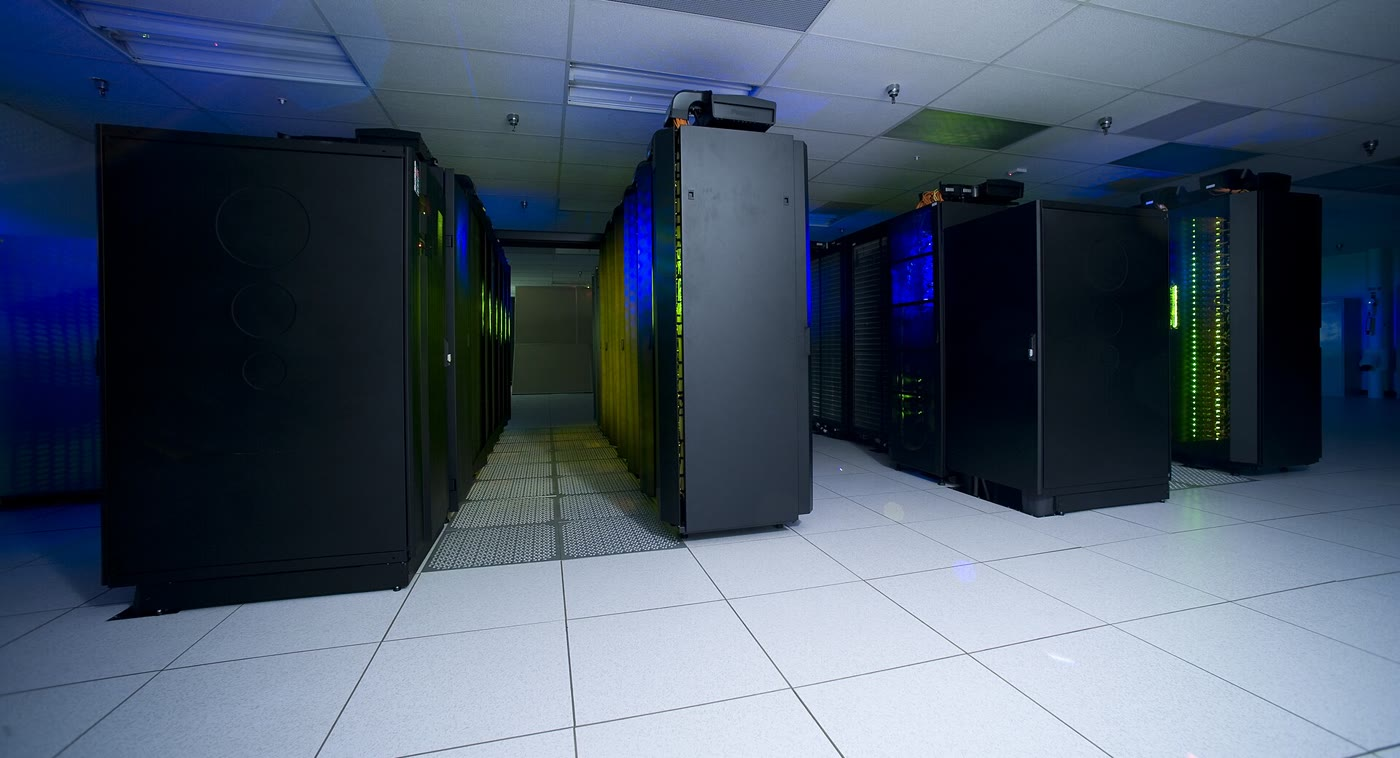
\includegraphics[width=0.7\linewidth]{images/book5/b3-nccs-supercomputer.jpg}

\par\smallskip{\small Rekken van een supercomputer bij het NASA Center for
Climate Simulation, Goddard Space Flight Center, in 2010 (NASA, publiek
domein). De vergelijkingen van een globaal model worden numeriek opgelost op zulke
hoogpresterende computers.}\label{fig:b3:climate-models:supercomputer}
\end{omfigure}
% ledger: photo:b3-nccs, ar6ch1:esm

\section{Modellen evalueren}\label{sec:b3:climate-models:evaluation}

Een model wordt getoetst aan het waargenomen klimaat; het probleem is dat het ook
op dat klimaat is afgesteld. Elke \omterm{def:b3:climate-models:gcm}{parametrisering} heeft parameters waarvan het
aanvaardbare bereik door de fysica en waarnemingen wordt bepaald, en terwijl de componenten
worden samengevoegd, verfijnen de modelleurs ze totdat het gesimuleerde klimaat voldoet aan
een reeks afstemdoelen: het gemiddelde klimaat --- bijvoorbeeld een gemiddelde temperatuur
dicht bij de waargenomen temperatuur onder de huidige zonnestraling --- regionale kenmerken, of
de trends van de historische periode. Pas dan wordt het model vrijgegeven voor de
modelvergelijkingen.
% ledger: ar6ch1:models, ar6ch1:parameterization, ar6ch1:large-ensembles

\begin{definition}[Modelvergelijkingsproject]\label{def:b3:climate-models:cmip}
Een \emph{modelvergelijkingsproject}\index{modelvergelijkingsproject}
is een gecoördineerde reeks experimenten --- dezelfde forcering, dezelfde
protocollen, dezelfde uitvoer --- uitgevoerd door veel modelleergroepen met
hun eigen modellen, zodat de resultaten vergeleken kunnen worden. Het Coupled Model
Intercomparison Project (CMIP) verloopt in opeenvolgende fasen; de zesde fase,
CMIP6, was een belangrijke bron van bewijs voor het zesde rapport.
\end{definition}

\begin{dated}{2021}
Van de 29 modelleergroepen van CMIP6 die rapporteerden hoe ze afstemden, stemden er 23
hun model niet af op de opwarming die in de historische periode is waargenomen, en
25 stemden hun ECS niet af: de gevoeligheid van de meeste modellen is een emergente
eigenschap, geen invoer. Gemiddeld hebben de CMIP6-modellen een hogere ECS en
TCR dan die van de vorige fase, en een bredere spreiding dan de bandbreedtes die het rapport
beoordeelde; in sommige modellen werd dit herleid tot de terugkoppeling van
de wolken op middelbare en hoge breedtegraden. Enkele van de gevoeligste modellen
reproduceren de waargenomen recente opwarming en de klimaten van het verleden minder
goed. Het rapport heeft daarom de bandbreedtes van ECS en TCR niet uit de modellen zelf overgenomen,
maar uit het begrip van de terugkoppelingsprocessen,
de instrumentele reeks, de klimaten uit het verleden en \omterm{def:b3:climate-models:evaluation}{emergente beperkingen}; het behandelt de gevoeligste modellen als leidraad voor
uitkomsten met lage waarschijnlijkheid en grote impact (\emph{hoge betrouwbaarheid}).
\end{dated}
% ledger: ar6ch1:models, ar6ch7:cmip6-sensitivity

\begin{definition}[Groot ensemble; emergente beperking]\label{def:b3:climate-models:evaluation}
Een \emph{groot ensemble}\index{groot ensemble} is een verzameling van vele simulaties
van één enkel model, met dezelfde forcering over dezelfde periode, die alleen
verschillen in hun begintoestanden. Een \emph{emergente
beperking}\index{emergente beperking} is een verband dat over een ensemble van
verschillende modellen heen wordt gevonden, tussen een waarneembare grootheid van het
huidige klimaat en een grootheid van het toekomstige, zoals de ECS; de
waargenomen waarde van de eerste beperkt dan de bandbreedte van de tweede.
\end{definition}

Het klimaat is chaotisch, zodat kleine verschillen in de begintoestand de
leden van een \omterm{def:b3:climate-models:evaluation}{groot ensemble} op verschillende paden brengen: de spreiding van de
leden meet de interne variabiliteit, en hun gemiddelde de geforceerde
respons. Grote ensembles van meerdere modellen ondersteunden het rapport. Een
\omterm{def:b3:climate-models:evaluation}{emergente beperking} heeft een fysische reden nodig. Bij enkele tientallen modellen
kunnen duizenden waarneembare grootheden worden getest, en sommige zullen toevallig met de
ECS correleren; het rapport hield die met een fysische basis aan, veel ervan
gaan over de wolken in de tropen, en waarschuwde dat een bias die alle
modellen van het ensemble delen, de methode ondermijnt.
% ledger: ar6ch1:large-ensembles, ar6ch7:emergent

\begin{inthelab}[Een modelleercentrum]
\begin{minipage}[t]{0.55\linewidth}\vspace{0pt}
In een klimaatmodelleercentrum is het model een programma dat geschreven en
onderhouden wordt door een team: atmosfeer, oceaan, zee-ijs en land zijn afzonderlijke
componenten die via een koppelaar fluxen aan hun grensvlakken uitwisselen. Voordat
een run begint, worden de forceringen van het experiment ingelezen --- de concentraties van
broeikasgassen, de aerosolen, het landgebruik volgens het protocol. De aardbol wordt
in stukken gesneden die de processoren van de supercomputer naast elkaar berekenen, en
een eeuw modelklimaat komt terug als een groot archief van
velden. De wetenschappers tonen ze op schermen, vergelijken ze met
reanalyses en satellietreeksen, en sturen de standaarduitvoer naar het
archief van het \omterm{def:b3:climate-models:cmip}{modelvergelijkingsproject}, waar andere groepen ze met hun eigen uitvoer vergelijken.
\end{minipage}\hfill
\begin{minipage}[t]{0.42\linewidth}\vspace{0pt}
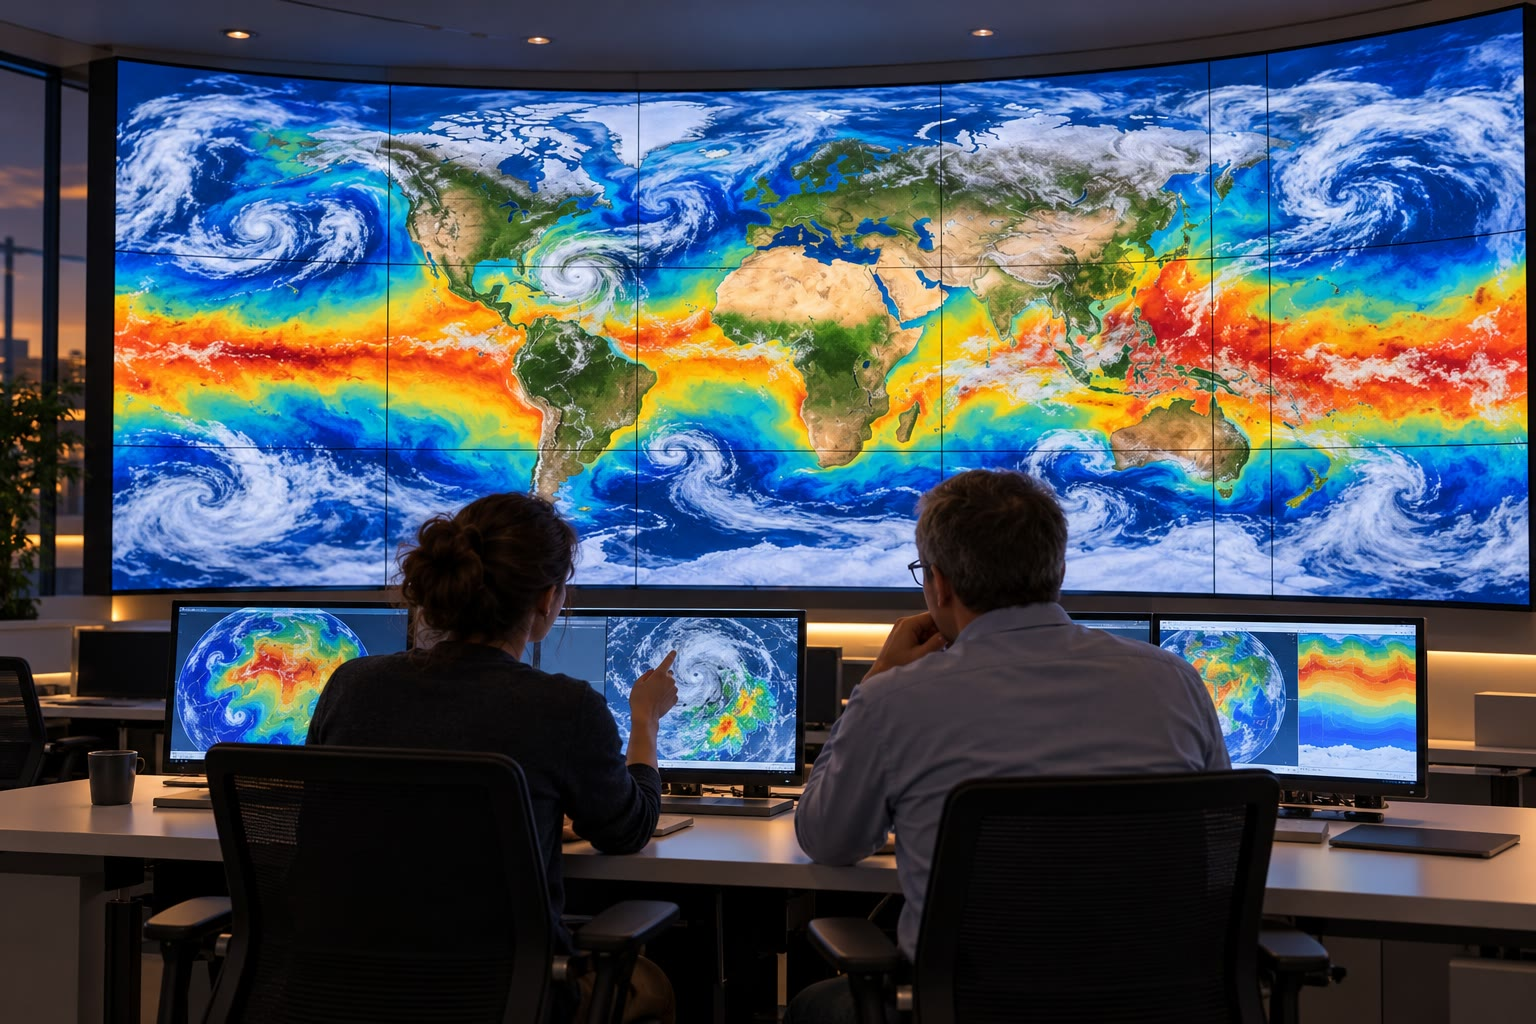
\includegraphics[width=\linewidth]{images/book5/ai/b3-model-centre.jpg}

{\scriptsize Twee wetenschappers voor een wand van schermen met globale
velden van een modelrun. Door AI gegenereerde illustratie.}
\end{minipage}
\end{inthelab}
% ledger: ar6ch1:esm, ar6ch1:models

\section{Oefeningen}

\begin{exercise}[$\star$]\label{exo:b3:climate-models:1}
Budyko's uitgaande langgolvige stralingswet is $I = a + bT - (a_1 + b_1T)n$, met $a = 14.0$, $b =
0.14$, $a_1 = 3.0$, $b_1 = 0.10$, in \unit{kcal.cm^{-2}} per maand en $T$
in \unit{\celsius}. Bereken voor een bewolking $n = 0.5$ de waarden van $A$ en $B$, en
reken ze om naar \unit{W/m^2} en \unit{W.m^{-2}.\celsius^{-1}}, waarbij een
maand gelijk is aan een twaalfde van een jaar van 365.25 dagen. Welke uitgaande langgolvige straling geeft de wet bij
\qty{15}{\celsius}?
\end{exercise}
% ledger: budyko69:olr

\begin{exercise}[$\star$]\label{exo:b3:climate-models:2}
Met $Q = \qty{340}{W/m^2}$, $A = \qty{211.9}{W/m^2}$ en $B =
\qty{1.816}{W.m^{-2}.\celsius^{-1}}$, bereken de evenwichtstemperatuur
voor een albedo van 0.30 en van 0.31. Hoeveel koelt deze planeet af bij een stijging
van de albedo met 0.01?
\end{exercise}

\begin{exercise}[$\star$]\label{exo:b3:climate-models:3}
Bereken de warmtecapaciteit per vierkante meter van een gemengde laag zeewater van
\qty{60}{m} diep, $\rho = \qty{1025}{kg/m^3}$ en $c_p = \qty{3992}{J.kg^{-1}.K^{-1}}$,
in \unit{J.m^{-2}.K^{-1}} en in \unit{W.yr.m^{-2}.K^{-1}}. Bereken de
responstijd van \cref{thm:b3:climate-models:response} voor $\lambda = -B =
\qty{-1.816}{W.m^{-2}.\celsius^{-1}}$ en voor $\lambda =
\qty{-1.33}{W.m^{-2}.\celsius^{-1}}$.
\end{exercise}
% ledger: teos10:cp0

\begin{exercise}[$\star$]\label{exo:b3:climate-models:4}
Voor het tweelaags model met $\lambda = \qty{-1.33}{W.m^{-2}.\celsius^{-1}}$,
$\gamma = \qty{0.62}{W.m^{-2}.\celsius^{-1}}$ en $F_{2\times} =
\qty{3.93}{W/m^2}$, bereken de ECS, de benaderde TCR $F_{2\times}/
(\gamma - \lambda)$, en hun verhouding.
\end{exercise}
% ledger: ar6sm7:two-layer, ipcc:erf-2xco2

\begin{exercise}[$\star\star$]\label{exo:b3:climate-models:5}
Neem in het nuldimensionale model uit de tekst een zonneconstante van
\qty{1340}{W/m^2}. Bepaal de drie evenwichten en de helling $N'(T)$ van de
netto flux bij elk daarvan; welke zijn stabiel?
\end{exercise}

\begin{exercise}[$\star\star$]\label{exo:b3:climate-models:6}
Verschuif de albedoramp uit de tekst: $\alpha = 0.62$ onder \qty{-20}{\celsius},
$0.30$ boven \qty{0}{\celsius}, lineair ertussen. Houd $A$ en $B$ gelijk. Bij welke
zonneconstante eindigt de warme tak, en met hoeveel procent ligt die
onder \qty{1360}{W/m^2}? Bij welke zonneconstante smelt de sneeuwbal?
Wat bepaalt de grootte van de drempel?
\end{exercise}

\begin{exercise}[$\star\star$]\label{exo:b3:climate-models:7}
Een modelplaneet met de parameters uit de tekst bevindt zich in de sneeuwbaltoestand.
(a)~Wat is de temperatuur bij de huidige zonneconstante? (b)~Met de Zon zoals hij is,
welke forcering $F$ brengt de temperatuur van de sneeuwbal omhoog tot
\qty{-10}{\celsius}? Hoeveel keer de forcering van een verdubbeling van
koolstofdioxide, \qty{3.93}{W/m^2}, is dat? (c)~Waar stelt de planeet zich in als de ijskap verdwenen is
en de forcering daarna wordt weggenomen?
\end{exercise}
% ledger: ipcc:erf-2xco2, hoffman17:hysteresis

\begin{exercise}[$\star\star$]\label{exo:b3:climate-models:8}
Model X, een verzonnen tweelaags model, heeft $C = 7.0$ en $C_d =
\qty{90}{W.yr.m^{-2}.\celsius^{-1}}$, $\gamma = 0.70$ en $\lambda =
\qty{-1.10}{W.m^{-2}.\celsius^{-1}}$. Bereken de twee tijdschalen exact
en met de benaderingen van \cref{thm:b3:climate-models:two-layer}, de
breuk $a_f$, de ECS en de benaderde TCR.
\end{exercise}

\begin{exercise}[$\star\star$]\label{exo:b3:climate-models:9}
In Budyko's model uit de tekst is $\bar T = \qty{12.81}{\celsius}$, $\beta =
\qty{3.74}{W.m^{-2}.\celsius^{-1}}$, de ijsgrens bij \ang{72}, $s = 1.221$
aan de evenaar en $0.506$ aan de pool, $\alpha = 0.30$ en $0.62$.
Bereken de temperatuur aan de evenaar en aan de pool, en de warmte
$\beta(T - \bar T)$ die het transport per
vierkante meter daar wegneemt, of aanvoert.
\end{exercise}

\begin{exercise}[$\star\star\star$]\label{exo:b3:climate-models:10}
Een planeet zonder ijs ($\alpha = 0.30$ overal) heeft het diffusieve
transport $D = -\mathcal D\,\partial_x[(1 - x^2)\partial_xT]$ en de
insolatie $s(x) = 1 + s_2P_2(x)$, $P_2 = (3x^2 - 1)/2$. (a)~Toon aan dat
$\partial_x[(1 - x^2)\partial_xP_2] = -6P_2$. (b)~Toon aan dat $T = T_0 +
T_2P_2(x)$ een stationaire oplossing is, met $T_0 = (Q(1 - \alpha) - A)/B$ en
$T_2 = Qs_2(1 - \alpha)/(B + 6\mathcal D)$. (c)~De insolatie van de
reanalyse geeft $s_2 = \num{-0.476}$. Wat zou zonder transport het temperatuurverschil zijn tussen
evenaar en pool? (d)~Welke $\mathcal D$ geeft
het waargenomen verschil, \qty{55.3}{\celsius}?
\end{exercise}
% ledger: data:b3-ncep, data:b5-ncep-air

\begin{exercise}[$\star\star\star$]\label{exo:b3:climate-models:11}
Schrijf de kwadratische vergelijking van \cref{thm:b3:climate-models:two-layer} als $r^2 -
\Sigma r + \Pi = 0$ en toon aan dat, als $4\Pi \ll \Sigma^2$, de wortels dicht bij
$\Sigma$ en $\Pi/\Sigma$ liggen. (b)~Voor een forcering $F = kt$ die lineair stijgt,
toon aan dat zodra $t \gg \tau_f$ en zolang $T_d$ klein blijft,
geldt $T \approx kt/(\gamma - \lambda)$; leid daaruit de benaderde TCR af. (c)~Controleer
de getallen uit de tekst: $\Sigma$, $\Pi$, de twee tijdschalen en de
verhouding $4\Pi/\Sigma^2$.
\end{exercise}
% ledger: ar6sm7:two-layer

\begin{exercise}[$\star\star\star$]\label{exo:b3:climate-models:12}
Een verzonnen ensemble van acht modellen geeft een waarneembare grootheid $X$ van het
huidige klimaat en hun ECS:
\begin{center}
\begin{tabular}{l*{8}{c}}
\hline
$X$ & 0.2 & 0.5 & 0.6 & 0.8 & 1.0 & 1.1 & 1.3 & 1.5\\
ECS (\unit{\celsius}) & 2.3 & 2.7 & 3.1 & 3.2 & 3.8 & 3.9 & 4.4 & 4.6\\
\hline
\end{tabular}
\end{center}
(a)~Bereken het gemiddelde en de standaardafwijking van de ECS van het
ensemble. (b)~Pas ECS $= a + bX$ aan met de kleinste kwadraten; bereken de correlatie
en de standaardafwijking van de residuen. (c)~De waargenomen $X$ is $0.7
\pm 0.1$. Welke ECS geeft de beperking, en met welke spreiding?
(d)~Wat zou je deze beperking doen wantrouwen?
\end{exercise}
% ledger: ar6ch7:emergent

\section{Probleem: Hoe dicht bij een sneeuwbal?}

\begin{problem}[{Weekendprobleem --- evenwichten, stabiliteit en de
verijzingsdrempel van een modelplaneet}]
\label{pb:b3:climate-models:1}
Een modelplaneet heeft de huidige zonneconstante $S_0 = \qty{1360}{W/m^2}$ en de
OLR-wet $A + BT$ met $A = \qty{211.9}{W/m^2}$ en $B =
\qty{1.816}{W.m^{-2}.\celsius^{-1}}$. Het albedo is 0.62 onder
\qty{-10}{\celsius}, 0.30 boven \qty{+10}{\celsius}, daartussen lineair, en
de oppervlaktewarmtecapaciteit $C = \qty{8.1}{W.yr.m^{-2}.\celsius^{-1}}$. Neem
$\sigma = \qty{5.670e-8}{W.m^{-2}.K^{-4}}$.

\medskip\noindent\textbf{Deel I --- De planeet in evenwicht.}
\begin{enumerate}
\item Bereken het gemiddelde zonlicht $Q_0$ per vierkante meter van de planeet, en
  verklaar de factor.
\item Bereken het geabsorbeerde zonlicht bij een albedo van 0.30, en de OLR bij
  \qty{15}{\celsius}.
\item Bereken het warme evenwicht.
\item Bereken het sneeuwbalevenwicht, en controleer dat het op de
  ijstak ligt.
\item Bereken het derde evenwicht, op de albedoramp.
\item Bereken de emissietemperatuur die het geabsorbeerde zonlicht
  als zwarte straler terug de ruimte in stuurt, en vergelijk die met het warme evenwicht.
\end{enumerate}

\medskip\noindent\textbf{Deel II --- Stabiliteit en tijd.}
\begin{enumerate}[resume]
\item Bereken de helling $N'(T)$ van de netto flux bij elk evenwicht, en zeg
  welke stabiel zijn.
\item Een kleine afwijking van het middelste evenwicht groeit als $\mathrm
  e^{t/\tau}$. Bereken $\tau$.
\item Bereken de responstijd van het warme evenwicht.
\item Een forcering van \qty{3.93}{W/m^2}, die van een verdubbeling van koolstofdioxide,
  wordt ingeschakeld. Bereken de opwarming in evenwicht, en vergelijk die met
  de voor het echte klimaat beoordeelde ECS.
\item Hoe lang doet het model erover om \qty{95}{\percent} van de
  opwarming te bereiken? Waarom doet het echte klimaat er langer over?
\end{enumerate}

\medskip\noindent\textbf{Deel III --- De zadel-knoopbifurcatie.}
\begin{enumerate}[resume]
\item Terwijl de Zon verzwakt, bij welke temperatuur komt het warme evenwicht
  samen met het middelste? Bereken $Q$ daar.
\item Bereken de zonneconstante bij de bifurcatie, en de daling ten opzichte van
  vandaag in procent.
\item Net eronder, waar gaat het klimaat naartoe? Bereken de temperatuur ervan.
\item Bereken de zonneconstante waarbij de sneeuwbal smelt, en de stijging
  ten opzichte van vandaag in procent.
\item Schets de lus die de temperatuur volgt wanneer $S_0$ wordt verlaagd
  onder de bifurcatie en teruggebracht naar \qty{1360}{W/m^2}.
\end{enumerate}

\medskip\noindent\textbf{Deel IV --- De ijslijn.} Geef de planeet
Budyko's latitudinale model, met $\beta = \qty{3.739}{W.m^{-2}.\celsius^{-1}}$,
een ijsalbedo van 0.62 poolwaarts van de ijslijn, 0.30 equatorwaarts, 0.50 bij
de rand, en de insolatie van de reanalyse:
\begin{center}
\begin{tabular}{lccccccc}
\hline
breedtegraad & \ang{0} & \ang{30} & \ang{40} & \ang{47.5} & \ang{55} & \ang{60} & \ang{72}\\
$s(x_s)$ & 1.2211 & 1.0730 & 0.9647 & 0.8688 & 0.7650 & 0.6947 & 0.5643\\
$F(x_s)$ & 0 & 0.5865 & 0.7324 & 0.8192 & 0.8863 & 0.9205 & 0.9738\\
\hline
\end{tabular}
\end{center}
\begin{enumerate}[resume]
\item Bereken, met de ijslijn bij \ang{72}, het gemiddelde albedo $\bar\alpha$
  en de gemiddelde temperatuur $\bar T$.
\item Bereken de kritieke temperatuur $T_c$ die de rand op
  \ang{72} vandaag legt, en vergelijk die met de reanalyse, \qty{-15.8}{\celsius}.
\item Bereken de teller van $Q(x_s)$ in \cref{prop:b3:climate-models:iceline}
  en de verhouding $\beta/B$.
\item Bereken $Q(x_s)/Q_0$ voor de ijslijn bij \ang{30}, \ang{40},
  \ang{47.5}, \ang{55} en \ang{60}.
\item Waar ligt het minimum van deze waarden? Welke ijslijnen zijn stabiel?
\item Welke andere ijslijn laat het model toe bij de huidige Zon, en is
  die stabiel? Is de sneeuwbal vandaag mogelijk? (Gebruik de kolom \ang{0}.)
\item Vergelijk de drempel van het latitudinale model met die van Deel~III
  en met Budyko's \qty{1.6}{\percent}, en de breedtegraad van het ijs bij de
  drempel met zijn \ang{50}.
\item Geef, op twee significante cijfers, de daling van de zonneconstante, in
  procent, die de modelplaneet verijst.
\end{enumerate}
\end{problem}
% ledger: nasa:solar-mean, data:b5-ncep-air, data:b3-ncep, budyko69:transport, budyko69:albedo, budyko69:threshold, ipcc:ecs, const:sigma
